\documentclass{beamer}
\usetheme{metropolis}
\usepackage{graphicx}
\usepackage{amsmath}
\usepackage{tcolorbox}
\title{Digital Signal Processing: COSC390}
\author{Jordan Hanson}
\institute{Whittier College Department of Physics and Astronomy}

\begin{document}
\maketitle

\begin{frame}{Unit 2.1 Outline}
\begin{enumerate}
\item \alert{\textbf{Introduction:} Types of filters} (reading: ch. 3, ch. 5)
\begin{itemize}
\item \alert{Butterworth}
\item \alert{Bessel}
\item \alert{Chebyshev}
\end{itemize}
\item \alert{LTI systems and their properties} (reading: ch. 5)
\item \alert{Convolution} (reading: ch. 7)
\begin{itemize}
\item \alert{Implementation with FFT}
\item \alert{Impulse and step response}
\end{itemize}
\end{enumerate}
Future lectures will cover:
\begin{enumerate}
\item SNR of filtered signals: SNR
\item Common filter kernels (moving average, windows)
\item Recursive filters
\item FIR and IIR definitions
\end{enumerate}
\end{frame}

\section{Introduction: Types of filters}

\begin{frame}{Introduction: Types of filters}
\small
Chapter 3 lists three types of anti-aliasing filters: Butterworth, Bessel, and Chebyshev.
Filters are examples of linear, time-invariant (LTI) devices
\begin{figure}
\centering
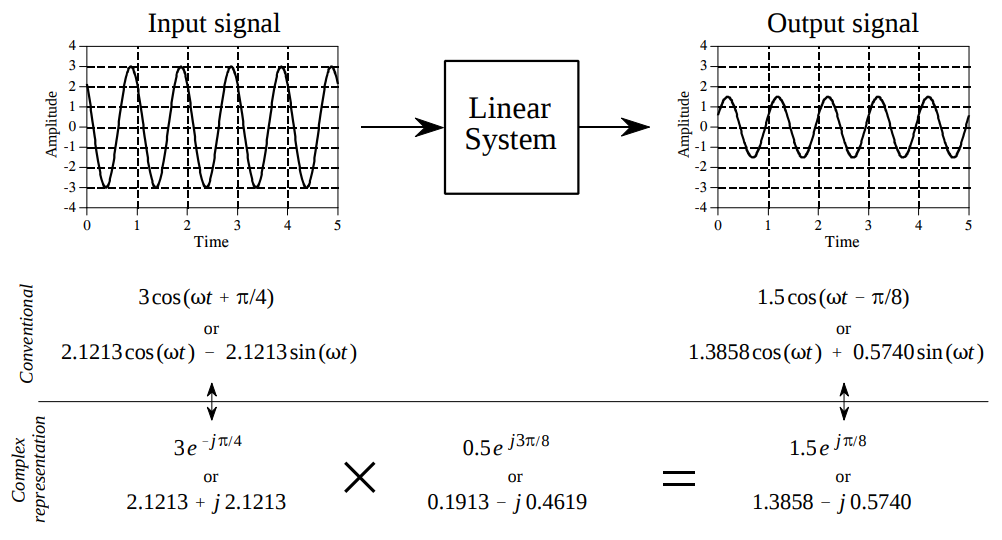
\includegraphics[width=0.8\textwidth]{figures/LTI1.png}
\caption{\label{fig:lti} A linear, time-invariant system has special properties encapsulated by the \textit{convolution operation.}}
\end{figure}
\end{frame}

\begin{frame}{Introduction: Types of filters}
\begin{figure}
\centering
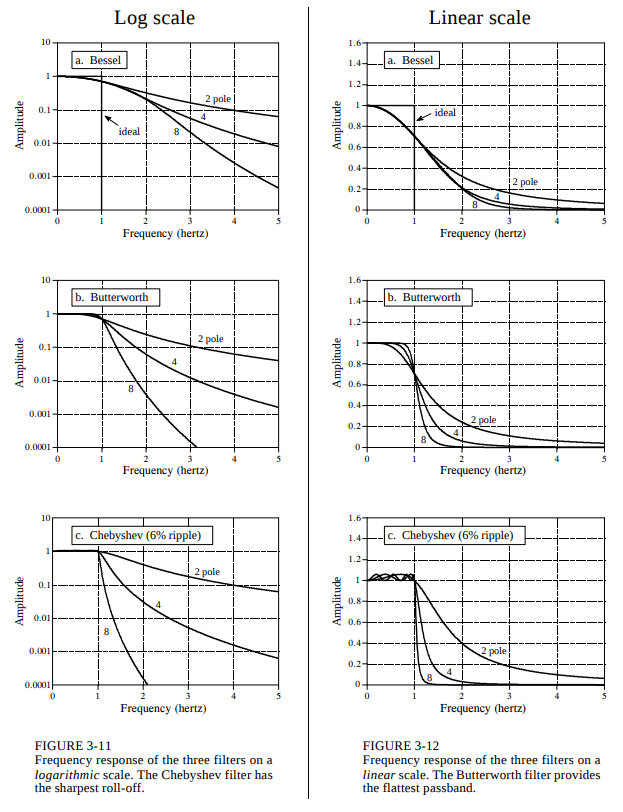
\includegraphics[width=0.5\textwidth]{figures/filters1.png}
\caption{\label{fig:filters1} Comparison of transfer function magnitudes.}
\end{figure}
\end{frame}

\begin{frame}{Introduction: Types of filters}
\begin{figure}
\centering
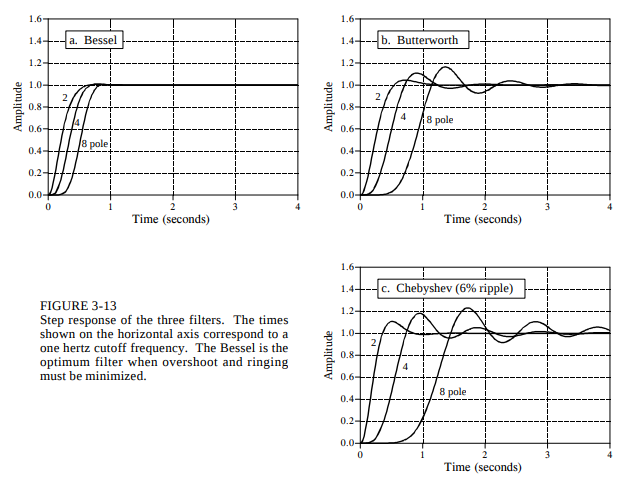
\includegraphics[width=0.75\textwidth]{figures/filters2.png}
\caption{\label{fig:filters2} Comparison of transfer function step responses.}
\end{figure}
\end{frame}

\begin{frame}{Introduction: Types of filters}
\begin{figure}
\centering
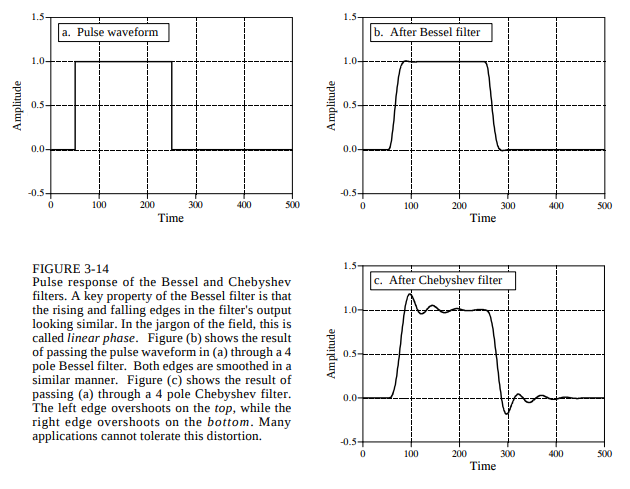
\includegraphics[width=0.75\textwidth]{figures/filters3.png}
\caption{\label{fig:filters3} Comparison of transfer function pulse responses.}
\end{figure}
\end{frame}

\begin{frame}{Introduction: Types of filters}
\small
The single-pole Butterworth transfer functions are derived from the single-pole RC filter circuit:
\begin{align}
H_{LP}(\omega) &= \frac{\omega_0}{\omega_0+j\omega} \\
H_{HP}(\omega) &= \frac{\omega}{\omega-j\omega_0}
\end{align}
\begin{itemize}
\item What frequency causes a singularity in the transfer functions?
\item What is the phase and group delay of this filter?
\end{itemize}
\end{frame}

\begin{frame}{Introduction: Types of filters}
\small
General expression for the transfer function of Butterworth filter (low-pass):
\begin{equation}
|H_{LP}(\omega)| = \frac{G_0}{\sqrt{1+\left(\frac{j\omega}{\omega_0}\right)^{2n}}} \label{eq:butter}
\end{equation}
The integer $n$ is the number of poles. $G_0$ is the \textit{gain}, and $\omega_0$ is the corner or cutoff frequency.
\begin{itemize}
\item Can we plot the poles in the complex plane?
\item What is the phase and group delay of this filter?
\end{itemize}
\end{frame}

\begin{frame}{Introduction: Types of filters}
\begin{figure}
\centering
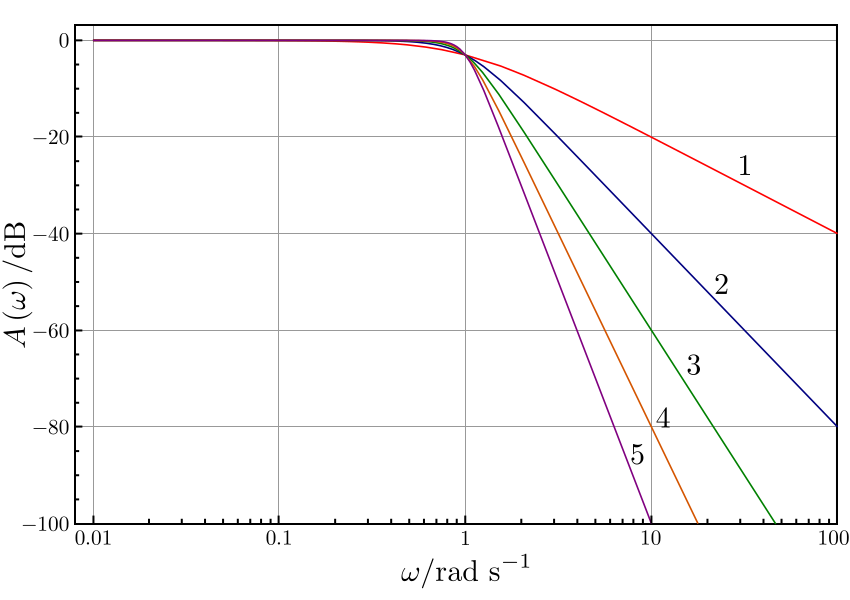
\includegraphics[width=0.75\textwidth]{figures/filtersb.png}
\caption{\label{fig:filters4} Gain of butterworth filters with $n$ poles.}
\end{figure}
\end{frame}

\begin{frame}{Introduction: Types of filters}
\small
The n-th order low-pass Bessel filter transfer function is a ratio of \textbf{reverse Bessel polynomials:}
\begin{equation}
H(\omega) = \frac{\theta_n(0)}{\theta_n(j\omega/\omega_0)}
\end{equation}
where the reverse Bessel polynomials $\theta_n(x)$ are given by
\begin{equation}
\theta_n(x) = \sum_{k=0}^{n} \frac{(n+k)!}{(n-k)!k!}\frac{x^{n-k}}{2^k}
\end{equation}
\begin{itemize}
\item What is $\theta_3$?
\item How do we turn this into a high-pass filter?
\item What are the pole locations of the 3rd-order Bessel filter?
\end{itemize}
\end{frame}

\begin{frame}{Introduction: Types of filters}
\small
The n-th order low-pass Chebyshev filter transfer function is
\begin{equation}
|H(\omega)| = \frac{1}{\sqrt{1+\epsilon^2 T_n^2(\omega/\omega_0)}}
\end{equation}
where the Chebyshev polynomials $T_n(x)$ are given by
\begin{align}
T_n(x) &= \cos(n\cos^{-1}(x)) ~~~|x| < 1 \\
T_n(x) &= \cosh(n\cosh^{-1}(x)) ~~~x \geq 1 \\
T_n(x) &= (-1)^n\cosh(n\cosh^{-1}(-x)) ~~~x \leq 1
\end{align}
\begin{itemize}
\item Can we plot $T_2(x)$ in Octave?
\item Pole locations are interesting (next slide).
\end{itemize}
\end{frame}

\begin{frame}{Introduction: Types of filters}
\begin{figure}
\centering
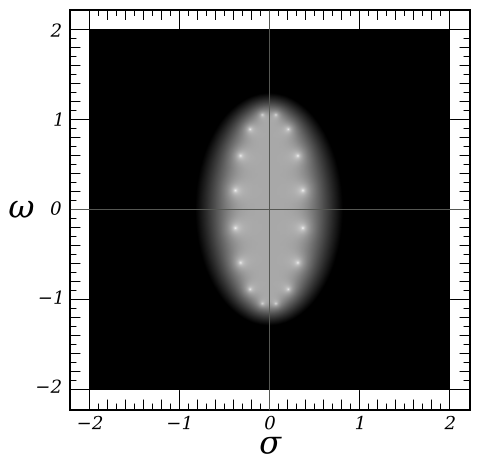
\includegraphics[width=0.5\textwidth]{figures/chebyshev.png}
\caption{\label{fig:filters5} Eight-pole Chebyshev filter in the complex plane. The poles form an ellipse, due to the trigonometric nature of the definition of Chebyshev polynomials.}
\end{figure}
\end{frame}

\begin{frame}[fragile]{Introduction: Types of filters}
\small
In the octave signal package, we can access the transfer functions of these filters:
\begin{verbatim}
pkg load signal;
[b1,a1] = butter(n,omega); %(e.g. include "high")
[b2,a2] = besself(n,omega);
[b3,a3] = cheby1(n,rp,omega); %rp pass-band ripple
x = (...); %data
y = filter(b1,a1,x);
\end{verbatim}
Use \textbf{help} function on these for more information.  The \textbf{filter} function is using the pole-zero information stored in the coefficients \textit{a} and \textit{b} to apply the transfer function to the data (more later).
\end{frame}

\section{Introduction: Types of filters, Octave programming example}

\begin{frame}[fragile]{Introduction: Types of filters}
\small
If you have the \textbf{signal} package, you can specify a n-th order butterworth filter with \textbf{butter} as above.  Otherwise, you can write a small function using Eq. \ref{eq:butter} for the digital response.
\begin{enumerate}
\item Create a white-noise sample (\textbf{randn}) of $10^4$ samples.  You can also specify a time vector of the same size.
\item Plot the spectrum of this noise using \textbf{fft}\footnote{See the \textbf{Aliasing.m} script in Unit 1}.).
\item \textbf{\alert{Filter}} the noise with a 2nd-order low-pass butterworth filter, at a cutoff frequency of 0.2 $f_s$. Either use the \textbf{filter} function and fft, or multiply in the Fourier domain.
\item \textbf{\alert{Filter}} the noise with a 2nd-order high-pass butterworth filter, at a cutoff frequency of 0.4 $f_s$.
\item Now do (3) then (4), and plot the spectrum.  Repeat for (4) then (3).  Do you see the same spectrum?
\end{enumerate}
\end{frame}

\section{LTI systems}

\begin{frame}[fragile]{LTI systems}
\textbf{Filters are LTI systems}.  Let's review the properties of LTI systems:
\begin{enumerate}
\item Continuous vs. discrete
\item Scaling property
\item Distributive property
\item Time-invariance (also causality)
\item Commutative property
\item Combination of properties
\end{enumerate}
\end{frame}

\begin{frame}{LTI systems}
\begin{figure}
\centering
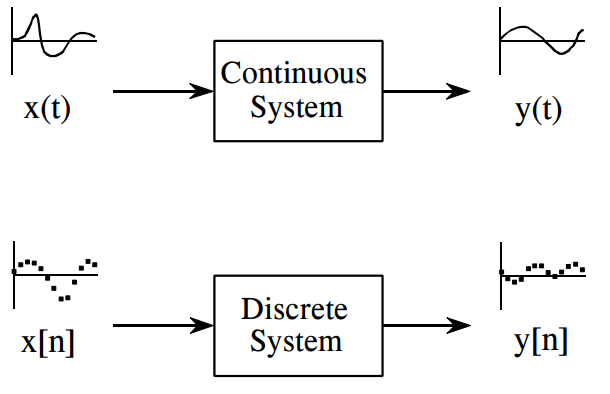
\includegraphics[width=0.5\textwidth]{figures/LTI2.png}
\caption{\label{fig:LTI2} A continuous LTI system response to continuous data, and a discrete LTI system response to discrete data.  All properties should hold both cases.}
\end{figure}
\end{frame}

\begin{frame}{LTI systems}
\begin{figure}
\centering
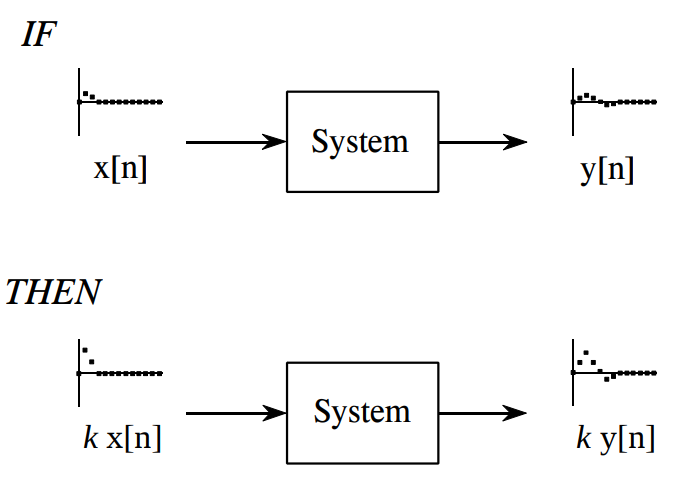
\includegraphics[width=0.5\textwidth]{figures/LTI3.png}
\caption{\label{fig:LTI3} Scaling: If the data is scaled by a real constant, the output should be scaled by a real constant.}
\end{figure}
\end{frame}

\begin{frame}{LTI systems}
\begin{figure}
\centering
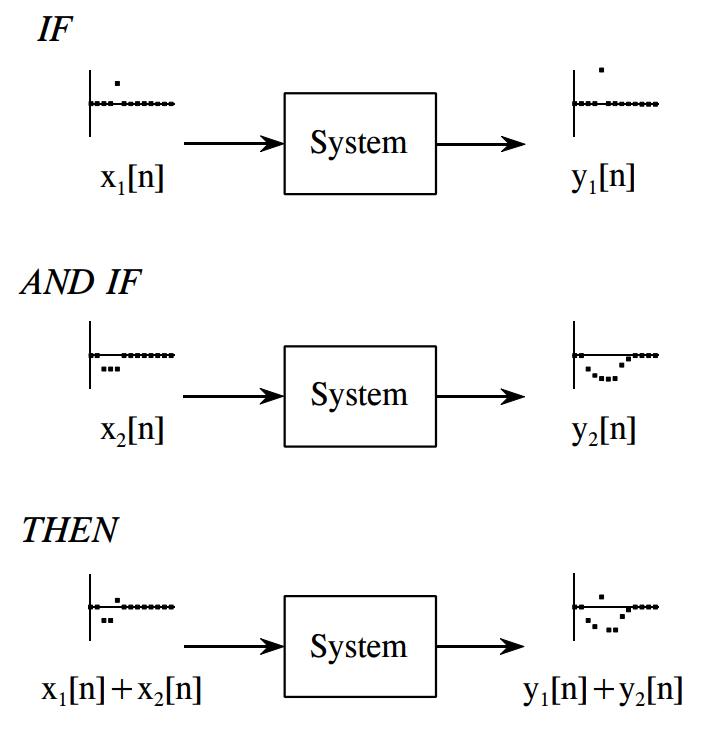
\includegraphics[width=0.5\textwidth]{figures/LTI4.png}
\caption{\label{fig:LTI4} Distributive property: the LTI system should respond to each signal separately.}
\end{figure}
\end{frame}

\begin{frame}{LTI systems}
\begin{figure}
\centering
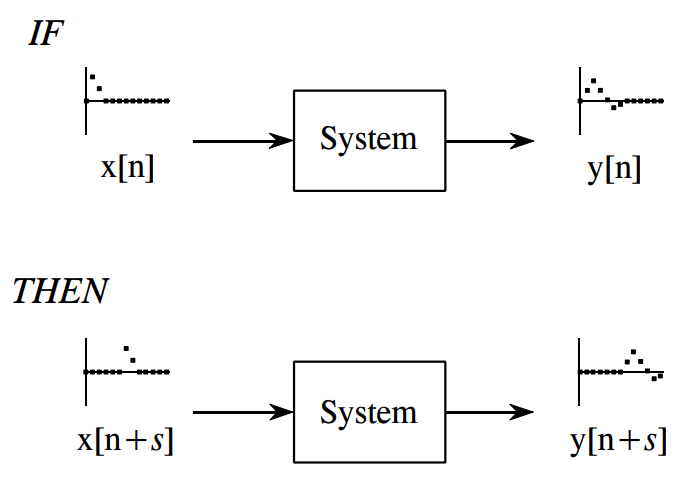
\includegraphics[width=0.5\textwidth]{figures/LTI5.png}
\caption{\label{fig:LTI5} Time-invariance: the LTI system should respond when the signal arrives, independent of global time. Also, the filter should not respond \textit{before} the signal arrives (causality).}
\end{figure}
\end{frame}

\begin{frame}{LTI systems}
\begin{figure}
\centering
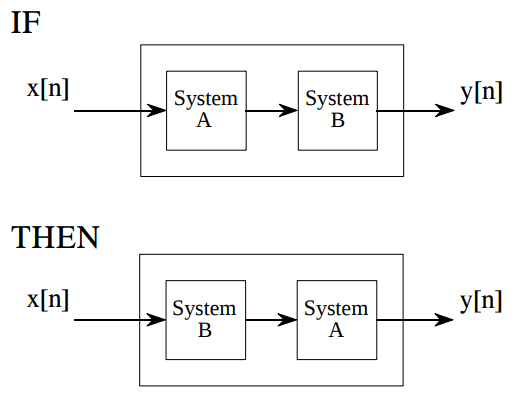
\includegraphics[width=0.5\textwidth]{figures/LTI6.png}
\caption{\label{fig:LTI6} Commutative property: the LTI system should not depend on the existence of previous systems.}
\end{figure}
\end{frame}

\begin{frame}{LTI systems}
\small
\begin{figure}
\centering
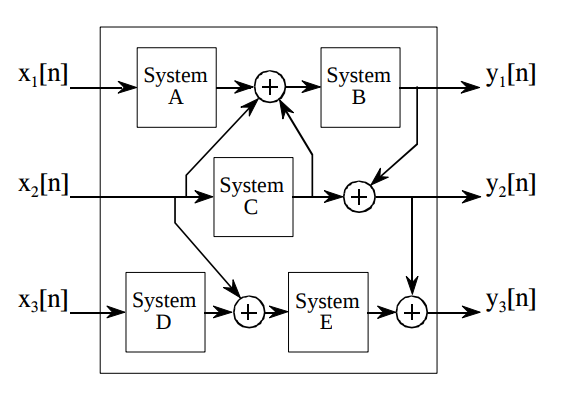
\includegraphics[width=0.5\textwidth]{figures/LTI7.png}
\caption{\label{fig:LTI7} Combination of properties: an LTI system may be built from a combination of LTI systems.}
\end{figure}
Suppose \textbf{A(x)}, \textbf{B(x)}, \textbf{C(x)}, \textbf{D(x)}, and \textbf{E(x)} represent \alert{operators} of LTI systems.  What is the formula for a) $y_1$, b) $y_2$ and c) $y_3$?  What is the the Fourier transform of the simplest output?
\end{frame}

\begin{frame}[fragile]{LTI systems}
\small
The \textbf{convolution} operator has all of the necessary properties of the LTI system operator.  The convolution of data streams $x_1$ and $x_2$:
\begin{verbatim}
x_1 = (...); %data1
x_2 = (...); %data2
y_1 = fft(x_1);
y_2 = fft(x_2);
Z_1 = y_1.*y_2;
result = real(ifft(Z_1));
\end{verbatim}
Or, in one line:
\begin{verbatim}
result = real(ifft(fft(x_1).*fft(x_2)));
\end{verbatim}
Or,
\begin{verbatim}
result = conv(x_1,x_2); %Pay attention to size
\end{verbatim}
\end{frame}

\section{LTI Systems: Programming with Octave}

\begin{frame}[fragile]{LTI Systems: Programming with Octave}
\small
The built-in Octave function \textbf{conv} for convolution produces two sizes, the full and the half-size.
\begin{verbatim}
x_1 = (...); %data
x_2 = (...); %data
y = conv(x_1,x_2);
size(y)
size(x_1)
size(x_2)
\end{verbatim}
Special case of \textbf{conv}:
\begin{verbatim}
y = conv(x_1,x_2,"same"); %default; "full"
size(y)
size(x_1)
size(x_2)
\end{verbatim}
\end{frame}

\begin{frame}[fragile]{LTI Systems: Programming with Octave}
\small
The \alert{unit-impulse} function $\delta$ is given by the identity:
\begin{equation}
x[n] \circ \delta[n] = x[n] \label{eq:impulse}
\end{equation}
Try the following in Octave:
\begin{verbatim}
clear; home; close;
function out = gauspulse(t,amp,mu,sigma)
    out = amp*exp(-0.5*((t-mu)/sigma).^2);
endfunction
t = linspace(0,10,10000);
r = zeros(size(t));
r(1000) = 1/sqrt(2); r(2500) = -1/sqrt(2);
x = gauspulse(t,1.0,5.0,0.2);
y = conv(r,x,"same");
plot(t,x,'color','black'); hold on;
plot(t,y,'color','blue');
sum(x.^2)/sum(y.^2)
\end{verbatim}
\end{frame}

\begin{frame}[fragile]{LTI Systems: Programming with Octave}	
\small
\begin{enumerate}
\item Does the output make sense? Why?
\item \textbf{Exercise}: Write Octave code that produces a sine wave.  Now write a transfer function that causes total destructive interferance.  When the sine wave is convolved with the transfer function, the output should be a DC level.
\item \textbf{Exercise}: Write a transfer function that doubles the amplitude.
\item \textbf{Thought experiment}: Could you write a transfer function that would double the frequency?  Why or why not?
\end{enumerate}
\end{frame}

\begin{frame}{Normal distribution}
\begin{tcolorbox}[colback=white,colframe=red!40!blue,title=Transfer Function]
\alert{The convolution of a \textbf{transfer function} with an input signal to an LTI system produces the output signal.  Mathematically, if $h(t)$ is the transfer function, $i(t)$ is the input signal, and $o(t)$ is the output:
\begin{equation}
o(t) = h(t) \circ i(t) = \int_{-\infty}^{\infty} h(\tau) i(t-\tau) d\tau
\end{equation}
The \textit{convolution theorem} also states that
\begin{equation}
o(t) = F^{-1} \lbrace H(\omega) I(\omega) \rbrace
\end{equation}
}
\end{tcolorbox}
\end{frame}

\begin{frame}[fragile]{LTI Systems: Programming with Octave}
\small
Consider the following function:
\begin{align}
h(t) &= \omega_0 \exp(-\omega_0 t) ~~~ t\geq 0 \\
h(t) &= 0 ~~~ t<0
\end{align}
\begin{enumerate}
\item What is the Fourier transform of $h(t)$?
\item Do you recognize this transfer function?
\item Write an Octave function that digitizes the time-dependent version of this transfer function.
\item Convolve with a sine wave of frequency $2\omega_0$.  What happens?
\end{enumerate}
\end{frame}

\begin{frame}[fragile]{LTI Systems: Programming with Octave}
\small
Let's repeat the exercise, but for \textit{high-pass} filtering.  Without knowing the time-domain equation for the response, how can we do this with transfer functions?
\begin{enumerate}
\item Consider taking the unit impulse signal \textit{minus} the low-pass component.  How do you add two transfer functions to get this to happen?
\item Convolve with a sine wave of a frequency less than the cutoff of the high-pass filter.  Do you see attenuation?
\end{enumerate}
\textbf{Normalization} of filters: (1) high-pass filters should have no gain at DC ($f=0$ Hz), and (2) Filters should conserve energy (amplitude squared) in the pass-band.  Let's ensure this by requiring
\begin{verbatim}
sum(h) = 1.0; %High-pass case
sym(h.^2) = 1.0; %Think about this one more...
\end{verbatim}
\end{frame}

\begin{frame}[fragile]{LTI Systems: Programming with Octave}
\small
\begin{figure}
\centering
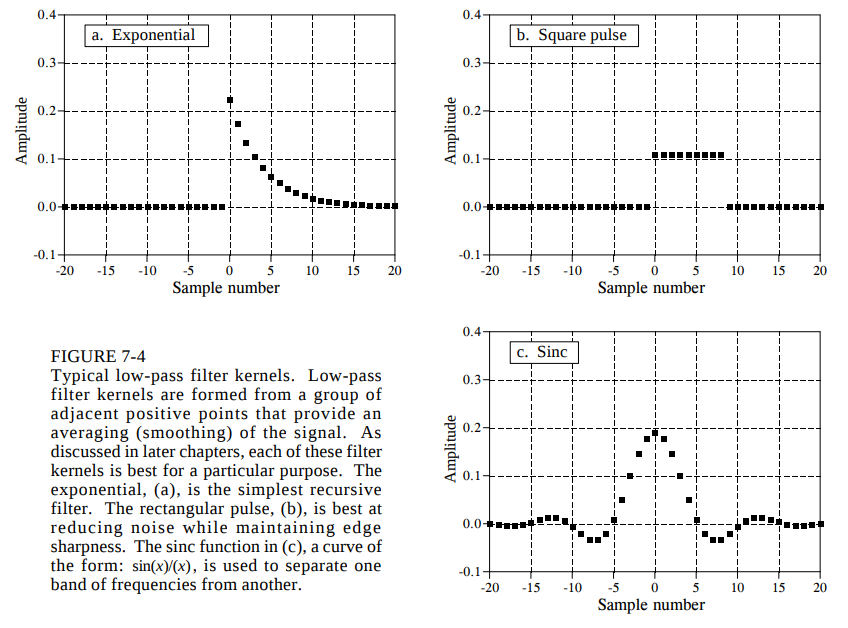
\includegraphics[width=0.75\textwidth]{figures/kernel1.png}
\caption{\label{fig:kernel1} Chapter 7: low-pass transfer functions, digitized.  Notice that they are wide, and positive.}
\end{figure}
\end{frame}

\begin{frame}[fragile]{LTI Systems: Programming with Octave}
\small
\begin{figure}
\centering
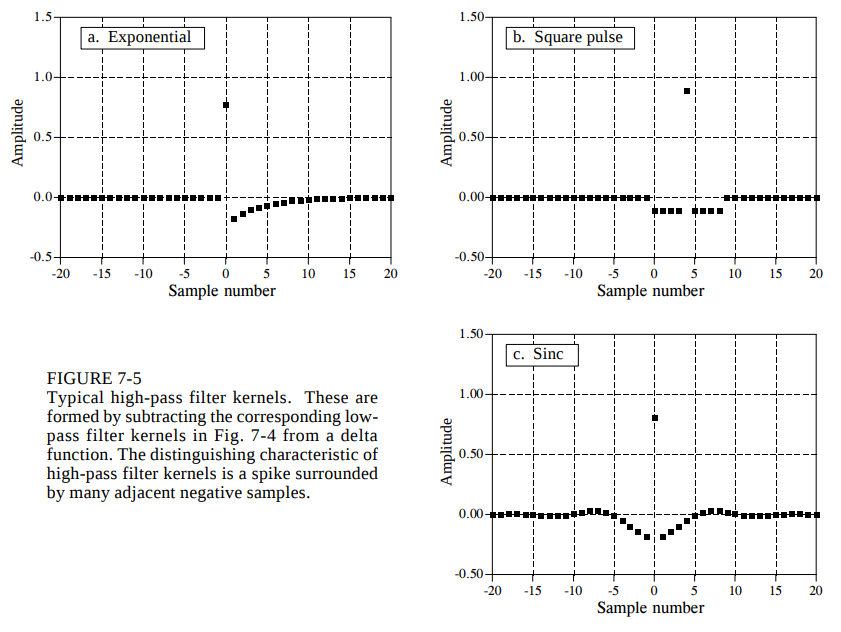
\includegraphics[width=0.75\textwidth]{figures/kernel2.png}
\caption{\label{fig:kernel2} Chapter 7: high-pass transfer functions, digitized.  Notice that they resemble the unit impluse minus a low-pass filter transfer function.}
\end{figure}
\end{frame}

\begin{frame}[fragile]{LTI Systems: Programming with Octave}
\small
\begin{figure}
\centering
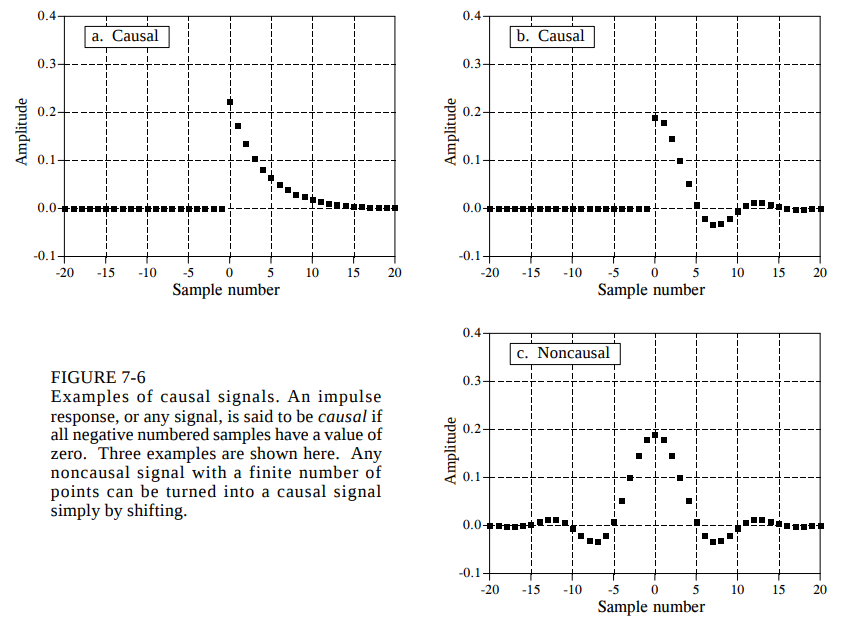
\includegraphics[width=0.75\textwidth]{figures/kernel3.png}
\caption{\label{fig:kernel3} Chapter 7: causal filters do not \textit{anticipate} the signal.}
\end{figure}
\end{frame}

\begin{frame}[fragile]{LTI Systems: Programming with Octave}
\small
\begin{figure}
\centering
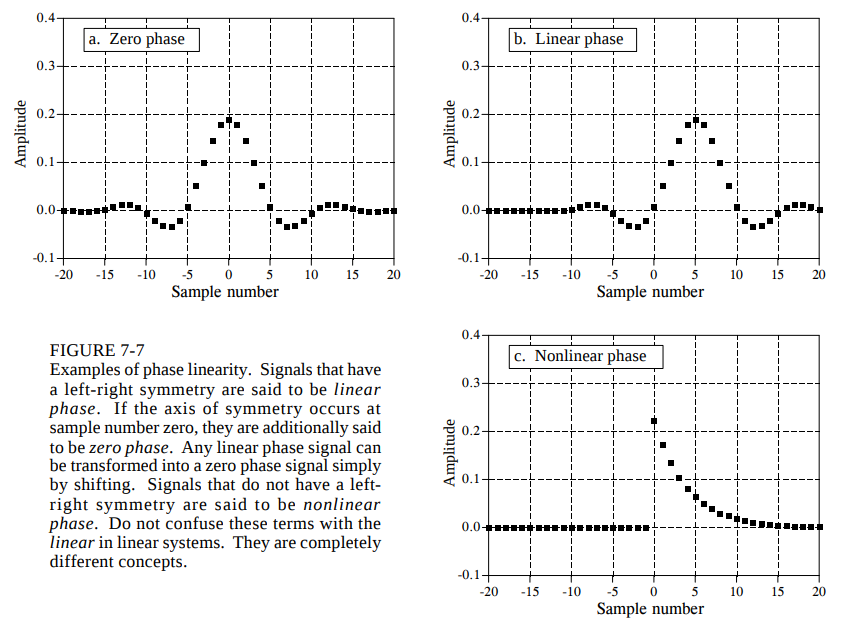
\includegraphics[width=0.75\textwidth]{figures/kernel4.png}
\caption{\label{fig:kernel4} Chapter 7: the phase of the transfer function can be related to the group delay.  What is meant by \textit{linear} phase, versus zero phase, in terms of group delay?}
\end{figure}
\end{frame}

\section{LTI Systems Application: RF filters and Johnson-Nyquist Noise}

\begin{frame}[fragile]{LTI Systems Application: RF filters and Johnson-Nyquist Noise}
\small
\textbf{Johnson-Nyquist noise} is the presence of random voltages across a circuit due to electron thermal fluctuations. Let $k_B$ be Boltzmann's constant\footnote{$k_B = 1.38 \times 10^{-23}$ m$^2$ kg s$^{-2}$ K$^{-1}$.}, $\Delta f$ be some bandwidth $f_{max} - f_{min}$ in frequency, $R$ be the resistance in Ohms at a temperature $T$ in Kelvin. The variance of the noise is
\begin{equation}
v^2_{rms} = 4 k_B T R \Delta f
\end{equation}
Let's write an Octave script to generate normally distributed noise with this \textit{variance.}  Make sure to define $\Delta f = f_{max} - f_{min}$.  Next, define a cosine or sine with frequency that is inside this bandwidth, and add it to the noise.  $SNR \approx 10$.
\begin{enumerate}
\item What happens to the SNR when you begin to filter the total signal, such that we keep the sinusoid intact?
\item Plot the SNR vs. cutoff frequency in your filter as you vary it.
\end{enumerate}
\end{frame}

\section{Special Topic: Impulse response of RF antennas}

\begin{frame}{Special Topic: Impulse response of RF antennas}
\small
A paper on RF antenna response for UHE neutrino research: \\ \url{https://doi.org/10.1016/j.astropartphys.2014.09.002}
\end{frame}

\end{document}
